\documentclass[a4paper,11pt]{article}

\usepackage{mathtools}
\usepackage{lipsum}
\usepackage{fullpage}
\usepackage{tabu}
\usepackage{wrapfig}
\usepackage{array,ragged2e,pst-node,pst-dbicons}
\usepackage{graphicx}

\title{Computer System II Networks Assignment}
\date{\today}
\author{James King}

\begin{document}
\maketitle

\begin{abstract}
\emph{The Travelling Salesman Problem is an example of the NP-Complete class of
problems; attempting to find the optimal solution by trying every possibility
would require an obscene amount of time for all but the smallest of input
sizes. This report describes two methods for finding decent solutions in a 
reasonable amount of time. The first is a type of stochastic gradient descent,
and the second is a nature inspired algorithm that models a simple ant colony.
A piece of analysis software was also produced to try and display each given
input in a form that is understandable to humans.}
\end{abstract}

\section{General Data Structures}
Each city graph, after being loaded from an input file, is stored in a 2D
integer array in such a way that the value in column $i$ and row $j$ is the
distance between city $i$ and city $j$. Representing the graph in this form
meant that checking the distance between two cities is a simple and fast
operation, and I hoped this would lead to my search algorithms being more time
efficient.

Routes are represented as fixed length one dimensional integer arrays, with
each value in the array being the index of the associated city. Each route also
has two numbers stored inside it that record the number of cities in the route
and the total cost of the route (the sum of the distances between each city in
the route). The value for the route cost is initially set to $-1$, and when it
is requested and its value is $-1$ it recalculates this cost. Additionally, any
operations that could change the length of the route set this value back to
$-1$, signalling that the value needs to be recalculated when next requested.

When an empty route is first created, the values in its city array are the
indexes of each city in ascending order. When the $i$th city is added to the
route, the relevant index is swapped with the value that was at the $i$th
position. This means that for a route of length $j$, all values in the array
from $j+1$ onwards are the indexes of cities that are not currently in the tour
and therefore can be selected to be added to the tour. I have also provided the
facility of selecting the $k$th best city from this subset, using the end of
the array as a buffer which is partially ordered until the city that is $k$th
best using a given comparison criteria is found.

\section{Algorithms}
\subsection{Algorithm A}
My first algorithm is a combined stochastic gradient descent and constructive
search. The algorithm starts with an empty route. For each step, a random city
from the set of unvisited cities is added to the end of the route. Next, a
hill climbing algorithm operates on the tour until no new improvements are
found. This process repeats, adding a new city every step, until the tour is
complete. Then this tour's length is calculated and compared with the shortest
found so far. If this is a new shortest tour, it is recorded and the whole
algorithm starts again.

The hill climbing method used in this algorithm is based around reversing
sections of the tour. To perform the reversal between two cities $T_i$ and
$T_j$ (where $T_i$ is the $i$th city in tour $T$), first the positions of $T_i$
and $T_j$ are swapped in the tour. Then $i$ is incremented by $1$, and $j$ is
decreased by $1$. The swapping and incrementing / decrementing process repeats
until $i \ge j$, which is when all cities between the initial two selected ones
have been reversed in place.

\begin{figure}
\begin{center}
\begin{tabular}{c}
\Large
\Circlenode[radius=4mm,linestyle=dashed]{f1start}{~}
\hskip 5mm
\Circlenode[radius=4mm]{f1A}{A} \ncline[linestyle=dashed]{f1start}{f1A}
\hskip 5mm
\Circlenode[radius=4mm]{f1B}{B} \ncline{f1A}{f1B}
\hskip 5mm
\Circlenode[radius=4mm]{f1C}{C} \ncline{f1B}{f1C}
\hskip 5mm
\Circlenode[radius=4mm]{f1D}{D} \ncline{f1C}{f1D}
\hskip 5mm
\Circlenode[radius=4mm]{f1E}{E} \ncline{f1D}{f1E}
\hskip 5mm
\Circlenode[radius=4mm]{f1F}{F} \ncline{f1E}{f1F}
\hskip 5mm
\Circlenode[radius=4mm]{f1G}{G} \ncline{f1F}{f1G}
\hskip 5mm
\Circlenode[radius=4mm,linestyle=dashed]{f1end}{~}
\ncline[linestyle=dashed]{f1G}{f1end}
\ncarc[arcangle=30,linestyle=dashed]{->}{f1B}{f1F}
\ncarc[arcangle=30,linestyle=dashed]{<-}{f1E}{f1A}
\\[1cm]
\Large
\Circlenode[radius=4mm,linestyle=dashed]{f2start}{~}
\hskip 5mm
\Circlenode[radius=4mm]{f2A}{A} \ncline[linestyle=dashed]{f2start}{f2A}
\hskip 5mm
\Circlenode[radius=4mm]{f2E}{E} \ncline{f2A}{f2E}
\hskip 5mm
\Circlenode[radius=4mm]{f2D}{D} \ncline{f2E}{f2D}
\hskip 5mm
\Circlenode[radius=4mm]{f2C}{C} \ncline{f2D}{f2C}
\hskip 5mm
\Circlenode[radius=4mm]{f2B}{B} \ncline{f2C}{f2B}
\hskip 5mm
\Circlenode[radius=4mm]{f2F}{F} \ncline{f2B}{f2F}
\hskip 5mm
\Circlenode[radius=4mm]{f2G}{G} \ncline{f2F}{f2G}
\hskip 5mm
\Circlenode[radius=4mm,linestyle=dashed]{f2end}{~}
\ncline[linestyle=dashed]{f2G}{f2end}
\end{tabular}
\end{center}
\caption{Segment of a tour before and after a reversal is applied between
	\emph{B} and \emph{E}, with the two new connections to be added represented
	by dashed arcs. The only connections that differ in cost to the original
	tour are the new connections from \emph{A} to \emph{E} and \emph{B} to
	\emph{F}.}
\end{figure}

The two cities to reverse between are chosen by checking every pair of cities
for the pair that would give the largest improvement to tour length if
reversed. The operation to find the change in tour length is made simple by the
fact that only two connections will be changed in a way that could affect the
tour length - the connections between the cities inside the swapped section are
only reversed but their length stays the same. The change in tour length is
therefore found like this:

$$(|\overrightarrow{{T_{i-1}}{T_i}}|
+ |\overrightarrow{{T_j}{T_{j+1}}}|)
- (|\overrightarrow{{T_{i-1}}{T_j}}|
+ |\overrightarrow{{T_i}{T_{j+1}}}|)$$

\noindent
Here $|\overrightarrow{{T_i}{T_j}}|$ is the distance between city $T_i$ and
$T_j$ as described by the city graph given as input.

Because of the nature of the reversal, some sets of pairs of cities would 
produce the same change in tour length when reversed. Pairs that would have
the same effect on tour length as others can be safely excluded to improve 
performance. I achieve this by picking the index $i$ of the first city, and the 
number of cities to reverse $c$, where $c \ge 2$ and
$c \le \frac{toursize}{2}$. This excludes swapping a city with itself (which
will never change the tour length) and any reversals that would return the same 
result as a previous one but with the whole tour in reverse.

The tour construction and reversal process is very fast, and because the
process is independent of any other systems related to the generation process
it may be easily threaded. This algorithm relies on being executed many, many
times to increase the probability of finding the optimal tour, and through
multithreading and other more general optimising techniques I improved the
speed of the algorithm to run thousands of tour tests a second. While the
algorithm may not be the smartest, by running it long enough it produced some
pretty small tour sizes. The algorithm keeps trying out new tours until no
better tours are found for a given number of attempts.

Initially the algorithm would only run the reversal improvement method after
the entire random tour was generated. This produced better results less
frequently and was actually slower despite running the improvement algorithm
only once per tour. The speed increase when improving after every new city
added is probably because the tour would require less reversal operations to
find a local minimum when the tour is larger (and the reversal algorithm is more
expensive) if the tour is constantly being maintained as it is built. However,
I am not certain that it is possible for the absolute optimal tour to be found
in every case when the tour is being improved as it is built whereas it is
trivial to see that finding the optimal tour is possible when only improving
after a random tour is built. In the end I decided to trade the possibility of
finding the optimal tour for finding sub optimal but decent tours more
frequently.

\subsection{Algorithm B}
My second algorithm is a constructive search using an Ant Colony heuristic.
The method places thousands of virtual ants at different starting positions on
the graph, which then wander between cities they have yet to visit until they
complete a tour. When a tour is complete, virtual pheromones are placed along
the route the ant took which influence other ants to take the paths along that
tour more often. Then the ant forgets which cities it has visited and starts
another tour.

The ants choose their next city to visit by first scoring each unvisited city
$C$ with the given criteria:

$$score = PW \times (PS[C] + 1.0)+(1.0 - PW) \times \frac{(CT + 1.0)}{PL[C]}$$

Here $PW$ is a random number between $0.0$ and $1.0$,
$PS[C]$ is the potency of the pheromones left on the path between
the ant's current city and city $C$, $CT$ is the number of tours
completed by any ant which was a new shortest tour, and $PL[C]$ is the
length between the ant's current city and city $C$.

After ranking each city in order by score, there is a random chance that the
ant will skip the best city and use the second best, and an either smaller
chance it will use the third best, and so on.

The amount of pheromone left when an ant completes a tour is given by:

$$pheromone = \frac{GraphCount}{TourCost - Minimum}$$

Here $GraphCount$ is the number of cities in the problem, $TourCost$ is the
total length of the tour, and $Minimum$ is the sum of the smallest cost from
each city to any neighbour. The total amount of pheromone between two cities is
also limited to being at most the number of fully completed tours that were new
shortest tours.

\begin{wrapfigure}{r}{0.42\textwidth}
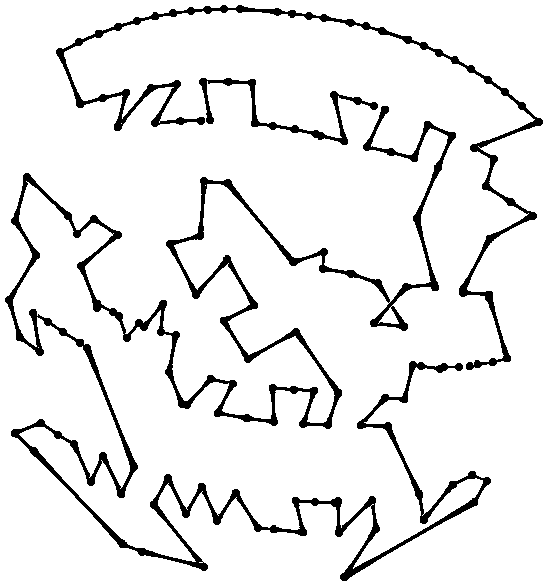
\includegraphics[width=0.4\textwidth]{175vis}
\caption{Visualisation of the 175 city graph with the current shortest route.}
\end{wrapfigure}

Like my first algorithm, this method can easily be threaded to improve speed.
Also, initially the ants would tend to stop improving the route found after
only a few iterations. I had written a simple tour visualiser that would
attempt to approximate the positions of cities in a graph assuming the path
costs given were euclidean distances, and I modified that visualiser to show
the routes each ant was taking at each step. This allowed me to repeatedly
modify my route selection and pheromone placement algorithms to try and get
the ants to experience more routes, as tested by viewing them with the
visualiser.

Admittedly I didn't spend as much time adjusting this algorithm as I did with
the first, mainly because the first algorithm produced very good results from
the start with relatively little effort. However, I expect that the ant colony,
given enough tweaking and thought, will be able to reliably produce better
results more frequently.

\section{Results Analysis}
The results displayed in Table 1 are the all-time lowest tour lengths
achieved by each algorithm. The table also shows the difference between the
results of the two algorithms, and the difference as a percentage of the
shortest tour's length.

\begin{table}[h]
\begin{center}
\begin{tabular}{| r | r  r  r |}
\hline
\textbf{City File} & \textbf{Result A} & \textbf{Result B} & \textbf{Difference} \\
\hline
\hline
SAfile012 & 56 & 56 & 0 (0.00\%) \\
SAfile017 & 1444 & 1444 & 0 (0.00\%) \\
SAfile021 & 2549 & 2549 & 0 (0.00\%) \\
SAfile026 & 1473 & 1473 & 0 (0.00\%) \\
SAfile042 & 1187 & 1188 & 1 (0.08\%) \\
SAfile048 & 12166 & 12505 & 339 (2.79\%) \\
SAfile058 & 25395 & 26027 & 632 (2.49\%) \\
SAfile175 & 21408 & 21774 & 366 (1.71\%) \\
SAfile180 & 1950 & 1950 & 0 (0.00\%) \\
SAfile535 & 48533 & 49061 & 528 (1.09\%) \\
\hline
\end{tabular}

\caption{Final results of both algorithms for each given city, and the
	difference between them.}
\end{center}
\end{table}

The first obvious thing to note is that both algorithms achieved the exact same
tour length for the first four tours. The fifth tour is almost also identical
for both algorithms, and in fact only differs by 1. Given the small size of the
graphs, this could be because the length found is the absolute optimum. Both 
algorithms find their respective minimum tours in very little time.

Tours for the graphs of size 48, 58 and 175 differ relatively greatly between
the two methods. As the graphs get larger, the number of possible tours
increases extremely rapidly and probability of an arbitrary tour being optimal
decreases rapidly too. For the first algorithm, this means that it is much less
likely to generate a random route that, when reduced, finds the global minimum
tour length and not just a local minimum. The second algorithm will have a
similar problem, in that it will tend towards a local minimum and then rest
there. As previously mentioned, the second algorithm should be able to explore
outside of any local minima found if the details of the method are optimised.
The first algorithm took a very long time to find its current lowest tours for
this graph, even though it can test many tours in a second. However, it found
results comparable to the quality that the second algorithm found in very
little time. The second algorithm would take a minute or two on the larger
graphs to reach a stable minimum, which would vary quite dramatically between
executions depending on what sequence the pseudo-random number generator would
produce.

The 180 node graph is an exceptional one. It has many paths between cities with
zero cost, which are apparently designed to act like ``dead ends'' in that a
Best First Search will attempt to follow these and end up at a city with the
only paths available having extremely high cost. Both of my methods seemed to
avoid this issue, however. An interesting difference between the two algorithms
is that the first took a few hours of execution over the course of many runs to 
arrive at its minimum, and yet the second finds the same result within a few 
seconds most of the time. However, this is not always the case; the second
method will occasionally find a tour with maybe double the length and not
improve, but this only seems to happen around half the time.

The last (and largest) graph 

\end{document}
